\documentclass[10pt]{article}
% Place this in your preamble (before \begin{document})
\usepackage{xcolor} % if not already loaded

\newcommand{\solution}{%
  \vspace{0.2in}%
  \noindent\textbf{\color{blue}Solution: }%
}

\def\Type{LessonCaelan}
\def\TypeNum{Lesson 15}
\def\TypeTitle{Net Change, Area \& Definite Integrals }
\def\Semester{Fall 2021} %Not Used 
\def\Course{MATH 1190 \& 1210}
\def\Targets{  {\bf\color{Fuchsia}I1} }

\usepackage{preambleDJ}

%\usepackage{ragged2e}


%%%%%%%%%%%% BEGIN DOCUMENT %%%%%%%%%%%%%%%
\begin{document}

\pagestyle{otherpages}
\thispagestyle{firstpage}
\vs{.65}

During our first lesson of the semester, we asked ``how are slope, rate of change, and net change related?". So far, we've discovered that slope and AROC are identical in a linear relationship, and that the slope of a tangent line is identical to IROC. However, we have not meaningfully related net change to any of these quantities.\\

Now that we've extensively developed a tool $-$ the derivative $-$ that can measure slopes \& IROC, we can begin to make better sense of the relationship between these quantities and net change. In this lesson, we will begin by using IROC estimating net change, and then introducing a new tool that can measure net change directly.\\

%%%%%%%%%%%%%%%%%%%%%%%%%%%%%%%%%%%%%%%%%%%%%%%%%%%%%%%%%%%%%%%%%%%%%%%%
{\example}\ltrm{\bf\color{Fuchsia}I1} Similarly to the online pre-class assignment, suppose the graph of the velocity $v(t)$ (in m/sec) of an object is given below, where $t$ is the time (in sec) since the object's movements were initially measured.
%
\begin{center}
    \begin{minipage}[t][1.8in][t]{0.25\textwidth}
    \,\\[-0.1in]
    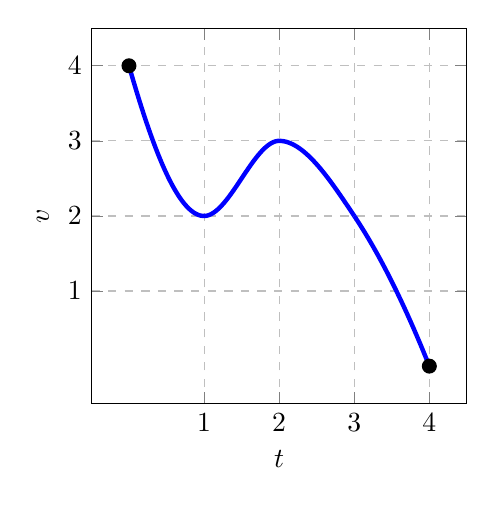
\begin{tikzpicture}
          \begin{axis}[
            xlabel = {$t$},
            ylabel = {$v$},
            xtick       = {1,2,3,4},
            xticklabels = {$1$,$2$,$3$,$4$},
            ytick       = {-2,-1,1,2,3,4,5,6},
            yticklabels = {$-2$,$-1$,$1$,$2$,$3$,$4$,$5$,$6$},
            samples     = 320,
            domain      = 0:4,
            xmin = -0.5, xmax = 4.5,
            ymin = -0.5, ymax = 4.5,
            width=2.5in,height=2.5in,
            grid=both, grid style=dashed
          ]
          \addplot[blue, ultra thick, mark=none, smooth, domain=0:1]  {4-7* x/2 + x^2 + x^3/2};
          \addplot[blue, ultra thick, mark=none, smooth, domain=1:2]  {7 - 12*x + 9*x^2 - 2*x^3};
          \addplot[blue, ultra thick, mark=none, smooth, domain=2:3]  {-7 + 12*x - 9/2* x^2 + x^3/2};
          \addplot[blue, ultra thick, mark=none, smooth, domain=3:4]  {2 + 3*x/2 - x^2/2};
          \filldraw (0,4) circle (2.5pt);
          \filldraw (4,0) circle (2.5pt);
         \end{axis}
    \end{tikzpicture}
    \end{minipage}
    %
    \quad
    %
    \begin{minipage}[t][1.8in][t]{0.68\textwidth}
    
    \begin{enumerate}
    \item[(a)] Estimate the net change $\Delta x$ in the position of the object between $2$ and $4$ seconds after measurements were intially taken.
    \end{enumerate}
    
    \end{minipage}
\end{center}
\solution
\blue
{Using the graph, approximate the area under the curve from $t=2$ to $t=4$. Visually estimating, we find
\[
\Delta x \approx 3.5 \text{ meters.}
\]}

\begin{enumerate}
\item[(b)] Given $t$ is assigned to the horizontal axis and $v$ is assigned to the vertical axis, how might we represent the quantity we computed in part (a) graphically? Sketch such a representation, and describe it in words below.

  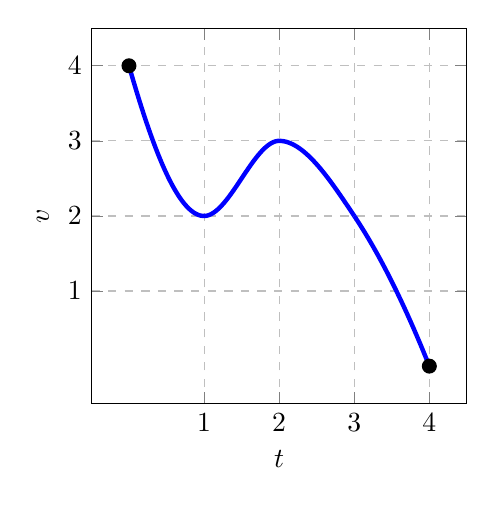
\begin{tikzpicture}
          \begin{axis}[
        %    axis y line = left,
        %    axis x line = bottom,
            xlabel = {$t$},
            ylabel = {$v$},
            xtick       = {1,2,3,4},
            xticklabels = {$1$,$2$,$3$,$4$},
            ytick       = {-2,-1,1,2,3,4,5,6},
            yticklabels = {$-2$,$-1$,$1$,$2$,$3$,$4$,$5$,$6$},
            samples     = 320,
            domain      = 0:4,
            %restrict y to domain=-5:5,
            xmin = -0.5, xmax = 4.5,
            ymin = -0.5, ymax = 4.5,
            width=2.5in,height=2.5in,
            grid=both, grid style=dashed
          ]
         %
         %\addplot[blue, ultra thick, mark=none, smooth] {4-x^2};
         %
        % \addplot[red, ultra thick, mark=none, smooth] coordinates{ (0,4) (1,2) (2,3)  (3,2) (4,0)};
               \addplot[blue, ultra thick, mark=none, smooth, domain=0:1]  {4-7* x/2 + x^2 + x^3/2};
          \addplot[blue, ultra thick, mark=none, smooth, domain=1:2]  {7 - 12*x + 9*x^2 - 2*x^3};
          \addplot[blue, ultra thick, mark=none, smooth, domain=2:3]  {-7 + 12*x - 9/2* x^2 + x^3/2};
          \addplot[blue, ultra thick, mark=none, smooth, domain=3:4]  {2 + 3*x/2 - x^2/2};
         %
         \filldraw (0,4) circle (2.5pt);
         %
         \filldraw (4,0) circle (2.5pt);
         \end{axis}
    \end{tikzpicture}

\solution
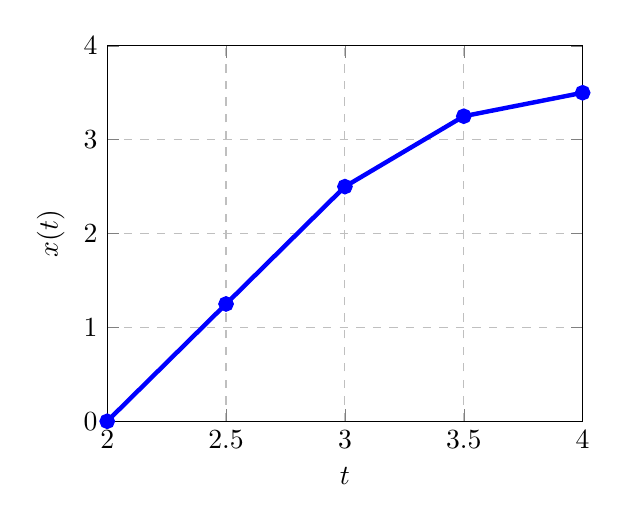
\begin{tikzpicture}
\begin{axis}[
    xlabel={$t$}, ylabel={$x(t)$},
    xmin=2, xmax=4,
    ymin=0, ymax=4,
    width=3in, height=2.5in,
    grid=both, grid style=dashed,
]

% Approximate accumulated area with piecewise linear points
\addplot[blue, ultra thick, mark=*] coordinates {
    (2,0)       % start at t=2
    (2.5,1.25)  % rough area estimate up to t=2.5
    (3,2.5)    % area up to t=3
    (3.5,3.25)  % area up to t=3.5
    (4,3.5)    % area up to t=4
};

% Mark final net change
%\filldraw[red] (axis cs:4,3.5) circle (2pt);
%\node[above, red] at (axis cs:4,3.5) {$\Delta x \approx 3.5$};

\end{axis}
\end{tikzpicture}

\blue{
Graphically, the net change in position corresponds to the area under the velocity curve between $t=2$ and $t=4$. 
%Positive areas indicate movement in the positive direction; negative areas indicate movement in the negative direction.}
}
\item[(c)] $x(t)$ represents the position of the object from the origin at time $t$.  Based on your answer in part (a), if the object was at position $10$ meters at $2$ seconds after measurements were initially taken, then approximately how far had the object travelled $4$ seconds after measurements were taken?

\solution
\blue{
We add the net change to the initial position:
\[
x(4) \approx x(2) + \Delta x \approx 10 + 3.5 = 13.5 \text{ meters.}
\]}

\end{enumerate}

%%%%%%%%%%%%%%%%%%%%%%%%%%%%%%%%%%%%%%%%%%%%%%%%%%%%%%%%%%%%%%%%%%%%%%%%
\newpage
{\exercise}\ltrm{\bf\color{Fuchsia}I1} The weight, $w$ (in pounds), of a baby  is described by a function $w(t)$ where $t$ represents weeks after birth.  Below is a graph of the {\em growth rate} $w'(t)$ (in pounds per week) of an infant's weight $t$ weeks after birth. 
\begin{center}
    \begin{minipage}[t][2in][t]{0.275\textwidth}
    \,\\[-0.1in]
    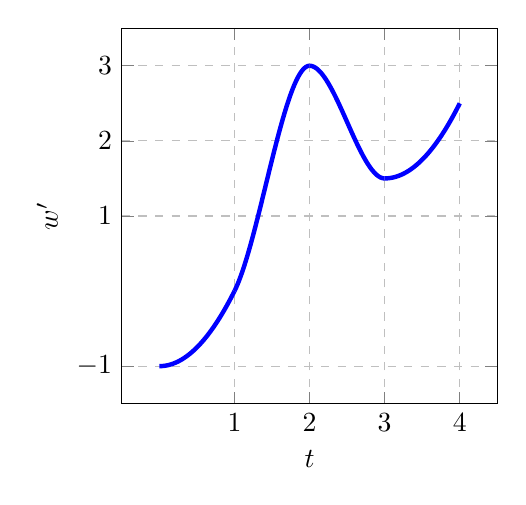
\begin{tikzpicture}
          \begin{axis}[
        %    axis y line = left,
        %    axis x line = bottom,
            xlabel = {$t$},
            ylabel = {$w'$},
            xtick       = {-2,-1,1,2,3,4,5,6},
            xticklabels = {$-2$,$-1$,$1$,$2$,$3$,$4$,$5$,$6$},
            ytick       = {-2,-1,1,2,3,4,5,6},
            yticklabels = {$-2$,$-1$,$1$,$2$,$3$,$4$,$5$,$6$},
            samples     = 320,
            domain      = -3:7,
            %restrict y to domain=-5:5,
            xmin = -0.5, xmax = 4.5,
            ymin = -1.5, ymax = 3.5,
            width=2.5in,height=2.5in,
            grid=both, grid style=dashed
          ]
         %
         % \addplot[blue, ultra thick, mark=none, smooth] coordinates{ (0,-1) (1,0) (2,3)  (3,1.5) (4,2.5)};
         %% In Mathematica, use ResourceFunction["CubicMonotonicInterpolation"][coords]. to find interpolating polynomial.
          \addplot[blue, ultra thick, mark=none, smooth, domain=0:1]  {x^2-1};
          \addplot[blue, ultra thick, mark=none, smooth, domain=1:2]  {7 - 20*x + 17*x^2 - 4* x^3};
          \addplot[blue, ultra thick, mark=none, smooth, domain=2:3]  {-39 + 54*x - 22.5*x^2 + 3* x^3};
          \addplot[blue, ultra thick, mark=none, smooth, domain=3:4]  {x^2-6*x+10.5};
         %
         \end{axis}
    \end{tikzpicture}
    \end{minipage}
    %
    \quad
    %
    \begin{minipage}[t][2in][t]{0.625\textwidth}
        \begin{enumerate}
        \item[(a)] Estimate the net change $\Delta w$ in the infant's weight from birth to $4$ weeks. Sketch rectangles whose areas represent your estimate. ({\it Note:} There are many correct answers to this prompt!)
        \end{enumerate}
    \end{minipage}
\end{center}
\vs{1}

\solution
\blue{Approximate the area under $w'(t)$ from $t=0$ to $t=4$. Suppose visually we get
\[
\Delta w \approx 5 \text{ pounds.}
\]
}





\begin{enumerate}


\item[(b)] Based on your answer in part (a), if the infant weighed 7 pounds at birth, then approximately how much did the infant weigh when the infant was 4 weeks old?

\solution
\blue{
Add the net change to the initial weight:
\[
w(4) \approx 7 + 5 = 12 \text{ pounds.}
\]
}
\end{enumerate}
\newpage
%%%%%%%%%%%%%%%%%%%%%%%%%%%%%%%%%%%%%%%%%%%%%%%%%%%%%%%%%%%%%%%%%%%%%%%%
{\bf\color{blue}Mini-lecture.} ({\it net change, area, and the definite integral})

\mpageTfour{.25}{.25}{.25}{.35}{
    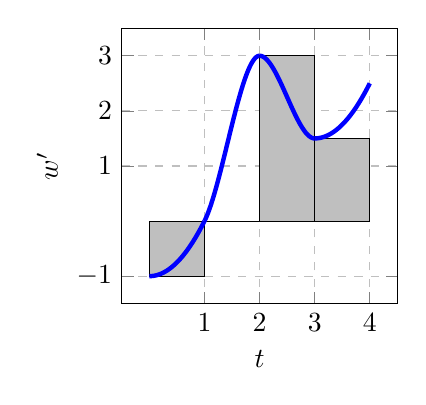
\begin{tikzpicture}
          \begin{axis}[
        %    axis y line = left,
        %    axis x line = bottom,
            xlabel = {$t$},
            ylabel = {$w'$},
            xtick       = {-2,-1,1,2,3,4,5,6},
            xticklabels = {$-2$,$-1$,$1$,$2$,$3$,$4$,$5$,$6$},
            ytick       = {-2,-1,1,2,3,4,5,6},
            yticklabels = {$-2$,$-1$,$1$,$2$,$3$,$4$,$5$,$6$},
            samples     = 320,
            domain      = -3:7,
            %restrict y to domain=-5:5,
            xmin = -0.5, xmax = 4.5,
            ymin = -1.5, ymax = 3.5,
            width=2in,height=2in,
            grid=both, grid style=dashed
          ]
         %
            \draw [fill=lightgray]  (3,1.5) rectangle (4,0); 
         \draw [fill=lightgray]  (2,3) rectangle (3,0); 
            \draw [fill=lightgray] (1,0) rectangle (2,0); 
            \draw [fill=lightgray] (0,-1) rectangle (1,0.0); 
         % \addplot[blue, ultra thick, mark=none, smooth] coordinates{ (0,-1) (1,0) (2,3)  (3,1.5) (4,2.5)};
         %% In Mathematica, use ResourceFunction["CubicMonotonicInterpolation"][coords]. to find interpolating polynomial.
          \addplot[blue, ultra thick, mark=none, smooth, domain=0:1]  {x^2-1};
          \addplot[blue, ultra thick, mark=none, smooth, domain=1:2]  {7 - 20*x + 17*x^2 - 4* x^3};
          \addplot[blue, ultra thick, mark=none, smooth, domain=2:3]  {-39 + 54*x - 22.5*x^2 + 3* x^3};
          \addplot[blue, ultra thick, mark=none, smooth, domain=3:4]  {x^2-6*x+10.5};
         %
         \end{axis}
    \end{tikzpicture}
    }{
    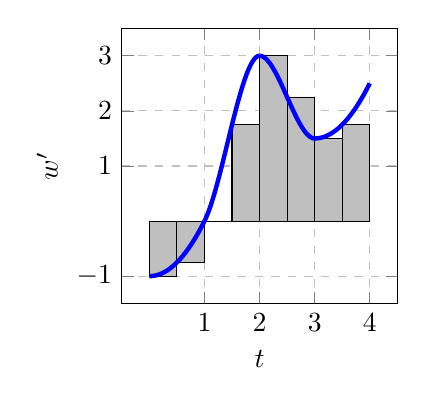
\begin{tikzpicture}
          \begin{axis}[
        %    axis y line = left,
        %    axis x line = bottom,
            xlabel = {$t$},
            ylabel = {$w'$},
            xtick       = {-2,-1,1,2,3,4,5,6},
            xticklabels = {$-2$,$-1$,$1$,$2$,$3$,$4$,$5$,$6$},
            ytick       = {-2,-1,1,2,3,4,5,6},
            yticklabels = {$-2$,$-1$,$1$,$2$,$3$,$4$,$5$,$6$},
            samples     = 320,
            domain      = -3:7,
            %restrict y to domain=-5:5,
            xmin = -0.5, xmax = 4.5,
            ymin = -1.5, ymax = 3.5,
            width=2in,height=2in,
            grid=both, grid style=dashed
          ]
         %
         \draw [fill=lightgray] (3.5,1.75) rectangle (4,0);
            \draw [fill=lightgray]  (3,1.5) rectangle (3.5,0); 
            \draw [fill=lightgray] (2.5,2.25) rectangle (3,0);
         \draw [fill=lightgray]  (2,3) rectangle (2.5,0); 
         \draw [fill=lightgray] (1.5,1.75) rectangle (2,0);
            \draw [fill=lightgray] (1,0) rectangle (1.5,0); 
            \draw [fill=lightgray] (.5,-.75) rectangle (1,0);
            \draw [fill=lightgray] (0,-1) rectangle (.5,0); 
         % \addplot[blue, ultra thick, mark=none, smooth] coordinates{ (0,-1) (1,0) (2,3)  (3,1.5) (4,2.5)};
         %% In Mathematica, use ResourceFunction["CubicMonotonicInterpolation"][coords]. to find interpolating polynomial.
          \addplot[blue, ultra thick, mark=none, smooth, domain=0:1]  {x^2-1};
          \addplot[blue, ultra thick, mark=none, smooth, domain=1:2]  {7 - 20*x + 17*x^2 - 4* x^3};
          \addplot[blue, ultra thick, mark=none, smooth, domain=2:3]  {-39 + 54*x - 22.5*x^2 + 3* x^3};
          \addplot[blue, ultra thick, mark=none, smooth, domain=3:4]  {x^2-6*x+10.5};
         %
         \end{axis}
    \end{tikzpicture}
    }{
        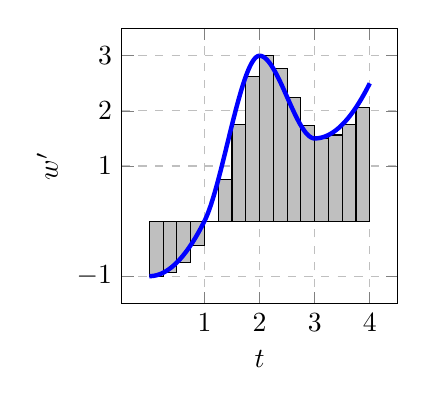
\begin{tikzpicture}
          \begin{axis}[
        %    axis y line = left,
        %    axis x line = bottom,
            xlabel = {$t$},
            ylabel = {$w'$},
            xtick       = {-2,-1,1,2,3,4,5,6},
            xticklabels = {$-2$,$-1$,$1$,$2$,$3$,$4$,$5$,$6$},
            ytick       = {-2,-1,1,2,3,4,5,6},
            yticklabels = {$-2$,$-1$,$1$,$2$,$3$,$4$,$5$,$6$},
            samples     = 320,
            domain      = -3:7,
            %restrict y to domain=-5:5,
            xmin = -0.5, xmax = 4.5,
            ymin = -1.5, ymax = 3.5,
            width=2in,height=2in,
            grid=both, grid style=dashed
          ]
         %
           \draw [fill=lightgray] (3.75,2.0625 ) rectangle (4,0);
         \draw [fill=lightgray] (3.5,1.75) rectangle (3.75,0);
           \draw [fill=lightgray] (3.25,1.5625 ) rectangle (3.5,0);
            \draw [fill=lightgray]  (3,1.5) rectangle (3.25,0); 
              \draw [fill=lightgray] (2.75,1.73438 ) rectangle (3,0);
            \draw [fill=lightgray] (2.5,2.25) rectangle (2.75,0);
              \draw [fill=lightgray] (2.25,2.76563 ) rectangle (2.5,0);
         \draw [fill=lightgray]  (2,3) rectangle (2.25,0); 
           \draw [fill=lightgray] ( 1.75,2.625) rectangle (2,0);
         \draw [fill=lightgray] (1.5,1.75) rectangle (1.75,0);
           \draw [fill=lightgray] ( 1.25,.75) rectangle (1.5,0);
            \draw [fill=lightgray] (1,0) rectangle (1.25,0); 
              \draw [fill=lightgray] ( .75,-.4375) rectangle (1,0);
            \draw [fill=lightgray] (.5,-.75) rectangle (.75,0);
             \draw [fill=lightgray] ( .25,-.9375) rectangle (.5,0);
            \draw [fill=lightgray] (0,-1) rectangle (.25,0); 
         % \addplot[blue, ultra thick, mark=none, smooth] coordinates{ (0,-1) (1,0) (2,3)  (3,1.5) (4,2.5)};
         %% In Mathematica, use ResourceFunction["CubicMonotonicInterpolation"][coords]. to find interpolating polynomial.
          \addplot[blue, ultra thick, mark=none, smooth, domain=0:1]  {x^2-1};
          \addplot[blue, ultra thick, mark=none, smooth, domain=1:2]  {7 - 20*x + 17*x^2 - 4* x^3};
          \addplot[blue, ultra thick, mark=none, smooth, domain=2:3]  {-39 + 54*x - 22.5*x^2 + 3* x^3};
          \addplot[blue, ultra thick, mark=none, smooth, domain=3:4]  {x^2-6*x+10.5};
         %
         \end{axis}
    \end{tikzpicture}
    }{
    \begin{flushright}
            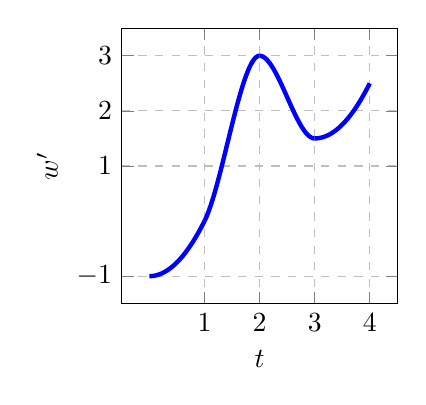
\begin{tikzpicture}
          \begin{axis}[
        %    axis y line = left,
        %    axis x line = bottom,
            xlabel = {$t$},
            ylabel = {$w'$},
            xtick       = {-2,-1,1,2,3,4,5,6},
            xticklabels = {$-2$,$-1$,$1$,$2$,$3$,$4$,$5$,$6$},
            ytick       = {-2,-1,1,2,3,4,5,6},
            yticklabels = {$-2$,$-1$,$1$,$2$,$3$,$4$,$5$,$6$},
            samples     = 320,
            domain      = -3:7,
            %restrict y to domain=-5:5,
            xmin = -0.5, xmax = 4.5,
            ymin = -1.5, ymax = 3.5,
            width=2in,height=2in,
            grid=both, grid style=dashed
          ]
         %
         % \addplot[blue, ultra thick, mark=none, smooth] coordinates{ (0,-1) (1,0) (2,3)  (3,1.5) (4,2.5)};
         %% In Mathematica, use ResourceFunction["CubicMonotonicInterpolation"][coords]. to find interpolating polynomial.
          \addplot[blue, ultra thick, mark=none, smooth, domain=0:1]  {x^2-1};
          \addplot[blue, ultra thick, mark=none, smooth, domain=1:2]  {7 - 20*x + 17*x^2 - 4* x^3};
          \addplot[blue, ultra thick, mark=none, smooth, domain=2:3]  {-39 + 54*x - 22.5*x^2 + 3* x^3};
          \addplot[blue, ultra thick, mark=none, smooth, domain=3:4]  {x^2-6*x+10.5};
         %
         \end{axis}
    \end{tikzpicture}
    \end{flushright}
    }
\vs{.5}

\important{The Definite Integral}
{
Let $a$ and $b$ be real numbers with $a<b$, and suppose $f$ is continuous on the interval $[a,b]$. The {\bf definite integral} of $f$ from $a$ to $b$ is denoted by \[\int_a^b f(x)\,dx\] and represents the \emph{\underline{\blue{net area}}} between the graph of $f$ and the $x$-axis from $a$ to $b$. If $f$ represents the rate of change of a quantity, then $\ds \int_a^b f(x)\,dx$ represents the \emph{\underline{\blue{net change}}} in the quantity as $x$ varies from $a$ to $b$.
}

\example Based on the definition of definite integral, write down a mathematical expression representing the net change $\Delta w$ in the infant's weight from birth to 4 weeks for the scenario in Exercise A, and indicate its unit.

\solution
\blue{$\displaystyle\int_0^4 w'(t)\,dt$ in pounds}

%%%%%%%%%%%%%%%%%%%%%%%%%%%%%%%%%%%%%%%%%%%%%%%%%%%%%%%%%%%%%%%%%%%%%%%%
{\exercise}\ltrm{\bf\color{Fuchsia}I1} Let $T'(t)$ represent the (instantaneous) rate of change (in $^{\circ}$C/day) of temperature in Charlottesville at a time $t$ (in days) during a particular week. 

\begin{enumerate}
\item[(a)] What are the units of $\ds \int_{1/2}^{3/2} T'(t)\,dt$? 

\solution
\blue{Units are $^\circ$C (temperature = (units of integrand) $\times$  (units of $t$ ), since integrating a rate of change over time gives the net change in temperature.}

\item[(b)] What does this integral represent in the given context?

\solution
\blue{
It represents the amount of change in temperature in celsius from noon of the first day to noon of the secon day.}

\item[(c)] If the temperature at noon on the first day of the week is $20^{\circ}$ C, then which of the following integral expressions represents the temperature at noon on the second day of the week?
\enumAA{
    \item $20+\ds \int_{1/2}^{3/2} T'(t)\,dt$ \quad \textcolor{blue}{\bf Correct}
    \item $20-\ds \int_{1/2}^{3/2} T'(t)\,dt$
    \item $\ds \int_{1/2}^{3/2} T'(t)\,dt-20$
    \item $\ds \int_{0}^{3/2} T'(t)\,dt$
    \item None of these options.
}
\end{enumerate}

%%%%%%%%%%%%%%%%%%%%%%%%%%%%%%%%%%%%%%%%%%%%%%%%%%%%%%%%%%%%%%%%%%%%%%%%
\newpage
{\exercise}\ltrm{\bf\color{Fuchsia}I1} The population of a country changes over time as people immigrate and emigrate. Suppose $f(t)$ gives the rate of change of the population $t$ years after officials began keeping records, in thousands per year. The graph of $f$ is given below.

\begin{minipage}[t]{0.3\textwidth}
\,\\[-0.1in]
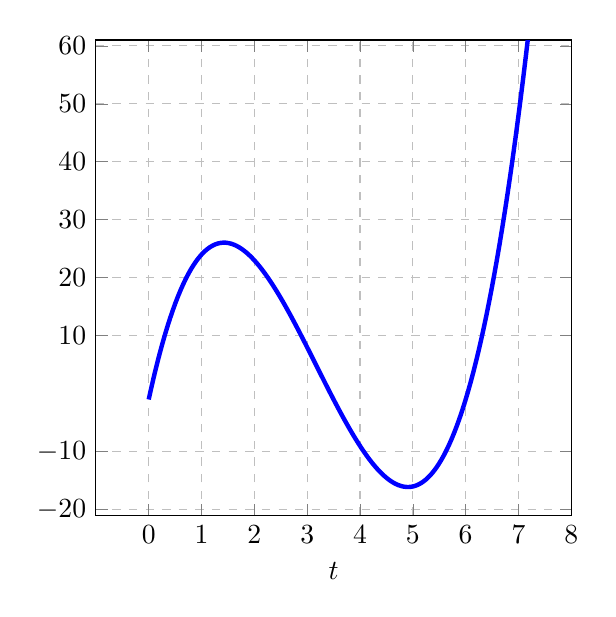
\begin{tikzpicture}
  \begin{axis}[
%    axis y line = left,
%    axis x line = bottom,
    xlabel = {$t$},
    %ylabel = { },
    xtick       = {0,1,2,3,4,5,6,7,8},
    xticklabels = {$0$,$1$,$2$,$3$,$4$,$5$,$6$,$7$,$8$},
    ytick       = {-20,-10,10,20,30,40,50,60},
    %yticklabels = {},
    samples     = 160,
    domain      = -1:3,
    restrict y to domain=-20:100,
    xmin = -1, xmax = 8,
    ymin = -21, ymax = 61,
    width = 3in, height=3in,
    grid=both, grid style=dashed
  ]
  \addplot[domain=0:8, blue, ultra thick] {-1+42*x-19*x^2+2*x^3};
\end{axis}
\end{tikzpicture}
\end{minipage}

\begin{enumerate}
\item[(a)] Interpret in words the meaning of each of the following in terms of the context described above, including units.
\begin{enumerate}
\item[i.] $f(1)=24$

\solution
\blue{The population is increasing at a rate of 24000 people per year at the end of year 1. \underline{Alternative Description:} If the population were to continue to change exactly as it did at the end of year 1, then the population would increase by 24000 people per year. (IROC)}

\item[ii.] $\ds \int_1^7 f(t)\,dt=36$

\solution
\blue{From the end of year 1 to the end of year 7, the population of this country grew by 36000 people.}

\end{enumerate}

\item[(b)] Use 3 rectangles of equal width to estimate $\ds \int_1^7 f(t)\,dt$. Sketch rectangles whose areas represent your estimate. Note: There are many reasonable ways to do this!


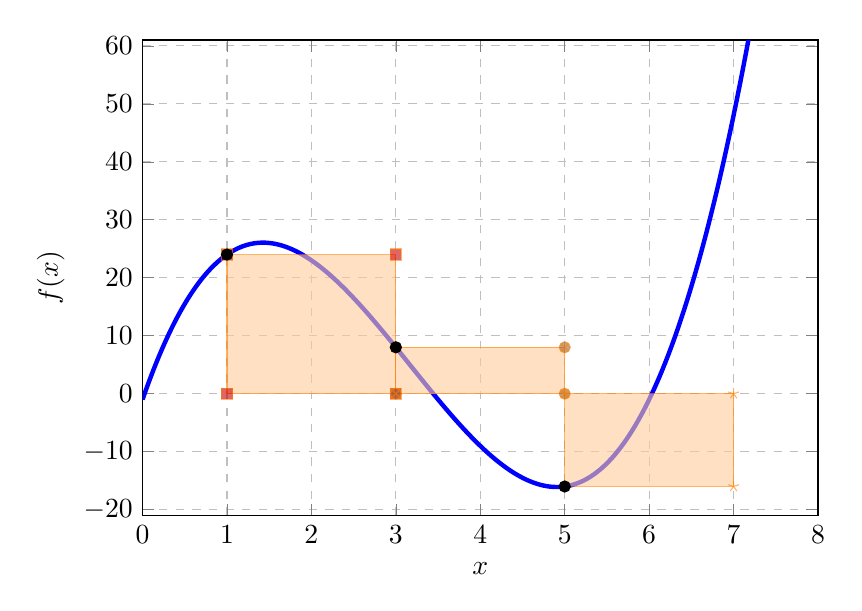
\begin{tikzpicture}
  \begin{axis}[
    xlabel={$x$},
    ylabel={$f(x)$},
    xmin=0, xmax=8,
    ymin=-21, ymax=61,
    xtick={0,1,2,3,4,5,6,7,8},
    ytick={-20,-10,0,10,20,30,40,50,60},
    grid=both,
    grid style=dashed,
    width=4in, height=3in,
    samples=200,
    domain=0:8,
  ]
    % Plot the function
    \addplot[blue, ultra thick, domain=0:8] {-1+42*x-19*x^2+2*x^3};

    % Left-endpoint rectangles (three rectangles on [1,7])
    % Rectangle 1: [1,3] height = f(1) = 24
    \addplot+[draw=orange, fill=orange!40, opacity=0.6] coordinates {(1,0) (1,24) (3,24) (3,0)} -- cycle;
    % Rectangle 2: [3,5] height = f(3) = 8
    \addplot+[draw=orange, fill=orange!40, opacity=0.6] coordinates {(3,0) (3,8) (5,8) (5,0)} -- cycle;
    % Rectangle 3: [5,7] height = f(5) = -16 (goes below x-axis)
    \addplot+[draw=orange, fill=orange!40, opacity=0.6] coordinates {(5,0) (5,-16) (7,-16) (7,0)} -- cycle;

    % Optional: mark left endpoints
    \addplot[mark=*, only marks] coordinates {(1,24) (3,8) (5,-16)};
  \end{axis}
\end{tikzpicture}





\solution

\blue{

Left endpoints: \quad \(x_0=1,\ x_1=3,\ x_2=5\). So, $\Delta x = 2$

\[
\begin{aligned}
f(1) & \approx 24,\\[6pt]
f(3) & \approx 8,\\[6pt]
f(5) & \approx-16.
\end{aligned}
\]

Left Riemann sum with 3 rectangles:
\[
L_3 = \sum_{i=0}^{2} f(x_i)\,\Delta x
= \Delta x\,[f(1)+f(3)+f(5)]
= 2\,[24 + 8 + (-16)]
= 2\cdot 16
= 32.
\]

\[
\boxed{L_3 = 32}
\]
}



\item[(c)] Suppose the population 1 year after officials began keeping records was $2000$. Write $-$ but do not solve $-$ an integral expression representing the number of people at time $t=4$.

\solution
\blue{
\[
P(4) = 2000 + \int_1^4 f(t)\, dt
\]
}
\end{enumerate}

%%%%%%%%%%%%%%%%%%%%%%%%%%%%%%%%%%%%%%%%%%%%%%%%%%%%%%%%%%%%%%%%%%%%%%%%
\newpage
{\bf\color{blue}Extra Practice 1.}\ltrm{\bf\color{Fuchsia}I1} A faucet is pouring water into a tank, which happens to have a small hole in the bottom. Suppose $r(t)$ is the rate at which the volume of water in the tank is changing, measured in gallons per hour, $t$ hours after the faucet is turned on.

\begin{enumerate}
\item[(a)] Interpret in words the meaning of each of the following in the given context, including units.
\begin{enumerate}
\item[i.] $r(2)=-1$

\solution
\blue{Two hours after the faucet is turned on, the water volume is decreasing at a rate of 1 gallon per hour.
\underline{Alternative Description:} If the volume of water were to continue to change exactly as it did two hours after the faucet is turned on, then the water volume would decrease by 1 gallon per hour. (IROC)}

\item[ii.] $\ds \int_1^3 r(t)\,dt$

\solution
\blue{This represents how much the volume of water (in gallons) in the tank changed from 1 hour to 3 hours after the faucet is turned on.}
\end{enumerate}

\item[(b)] Write a mathematical expression representing the following.
\begin{enumerate}
\item[i.] the net change (in gallons) in the amount of water in the bucket two hours after the faucet is turned on

\solution
\blue{
\[
\text{Net change from } t=0 \text{ to } t=2: \int_0^2 r(t)\, dt
\]
}

\item[ii.] the initial rate (in gallons per hour) at which the volume of water in the tank is changing   

\solution
\blue{
\[
r(0)
\]
}
\end{enumerate}

\item[(c)] Suppose the tank initially contains $1$ gallon of water. Write an integral expression representing the amount of water in the bucket $2$ hours after the faucet is turned on.

\solution
\blue{
\[
\text{Volume at } t=2: 1 + \int_0^2 r(t)\, dt
\]
}
\end{enumerate}

\end{document}
